\begin{scanpage}{0150}{132}
\begin{center}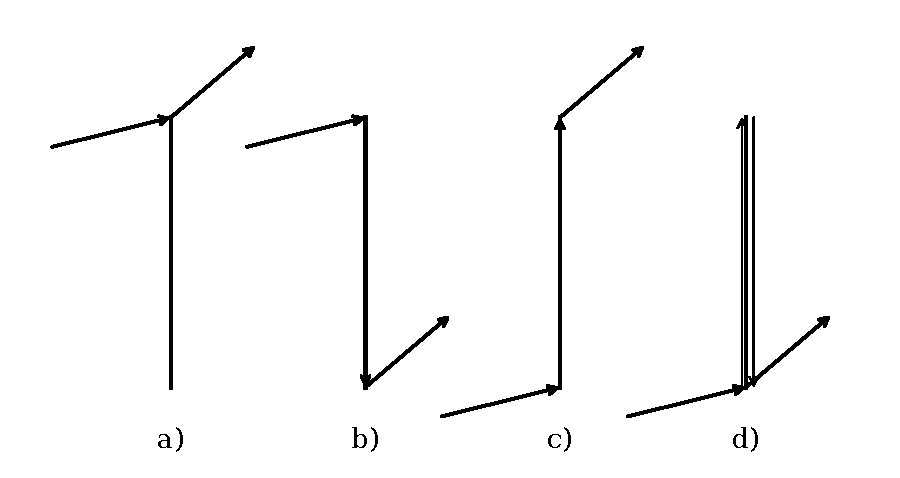
\includegraphics[width=.55\linewidth]{images/recreated/c-0150-fig.pdf}\par
Figure 48. The schematic diagram of the waves corresponding to the various terms in Equation (22.05).
\end{center}
$F(1,\alpha)$, $F(2,\alpha)$ will, as before, be described by the relationships (21.22), (21.23) and (22.13). The remaining functions in Equations (22.02) will be determined when $\pi/2<|\varphi|<\pi$ by the following equations:
\[
\left.\begin{aligned}G(1,\varphi)&=\frac2{\sqrt\pi}e^{-i\pi/4}\int_0^{\pm2\sqrt{ka}\sin(\pi/4+\varphi/2)}e^{iq^2}\,dq,\\
G(2,\varphi)&=\frac2{\sqrt\pi}e^{-i\pi/4}\int_0^{\mp2\sqrt{ka}\sin(\pi/4-\varphi/2)}e^{iq^2}\,dq,
\end{aligned}\right\}\tag{23.06}
\]
\[
\left.\begin{aligned}F(1,\varphi)&=\frac2{\sqrt\pi}e^{-i\pi/4}\Bigl[\int_0^{\pm2\sqrt{ka}\sin(\pi/4+\varphi/2)}e^{iq^2}\,dq\pm\frac{i}{4\sqrt{ka}}\frac{e^{2ika(1+\sin\varphi)}}{\sin(\pi/4+\varphi/2)}\Bigr],\\
F(2,\varphi)&=\frac2{\sqrt\pi}e^{-i\pi/4}\Bigl[\int_0^{\mp2\sqrt{ka}\sin(\pi/4-\varphi/2)}e^{iq^2}\,dq\mp\frac{i}{4\sqrt{ka}}\frac{e^{2ika(1-\sin\varphi)}}{\sin(\pi/4-\varphi/2)}\Bigr].
\end{aligned}\right\}\tag{23.07}
\]
\end{scanpage}
